% Intestazione
\fancyhead[L]{4 \hspace{0.2cm} Pianificazione} % Testo a sinistra

% Sezione 
\section{Pianificazione}
\label{sec:pianificazione}
Il gruppo \emph{SWEg Labs}\textsubscript{\textit{\textbf{G}}} ha deciso di strutturare il proprio progetto in modo sistematico, 
organizzando le attività secondo scadenze ben definite, indicate all'inizio di ogni sezione. Le attività saranno suddivise in base alla fase di revisione e per argomento, garantendo così un approccio strutturato e focalizzato sui diversi stadi del progetto.\\
Un \emph{Diagramma di Burndown}\textsubscript{\textit{\textbf{G}}} fornirà una rappresentazione grafica dell'avanzamento del lavoro nel tempo, facilitando il monitoraggio costante del progresso e la gestione delle risorse.\\
Questo strumento consentirà al team di mantenere una visione d'insieme sull’avanzamento del progetto e di apportare eventuali aggiustamenti per rispettare le tempistiche pianificate.
Verrà redatto durante ogni sprint un consuntivo dettagliato, che includerà sia i costi che le ore impiegate da ciascun membro del team. Tale analisi offrirà una chiara panoramica delle risorse investite e dei risultati ottenuti, rendendo possibile una valutazione complessiva dell’efficienza e dell’efficacia del progetto.
Il progetto del gruppo \emph{SWEg Labs} sarà suddiviso nelle seguenti fasi:
\begin{itemize}
    \item \textbf{Studio preliminare dei capitolati}: Analisi dei capitolati per valutare vantaggi e svantaggi di ciascuno, al fine di identificare quello che meglio si adatta alle competenze e agli interessi del gruppo, garantendo una scelta in linea con le esigenze progettuali.
    \item \textbf{\emph{Requirements and Technology Baseline}}\textsubscript{\textit{\textbf{G}}}: Definizione dei requisiti e delle tecnologie di base necessarie per il progetto.
    \item \textbf{\emph{Product Baseline}}\textsubscript{\textit{\textbf{G}}}: Sviluppo del prodotto secondo i requisiti definiti.
\end{itemize}

Questa suddivisione consentirà al gruppo di avanzare in modo ordinato, 
assicurando che ogni fase del progetto sia completata in maniera ottimale per garantire il massimo livello di qualità e soddisfazione del cliente.

\vspace{0.5cm}

\subsection{Studio preliminare dei Capitolati}
\begin{table}[h!]
    \centering
    \renewcommand{\arraystretch}{1.5} % Aumenta l'altezza delle righe
    \begin{tabularx}{\textwidth}{|X|X|X|}\hline
    \rowcolor[HTML]{FFD700} 
    \textbf{Data di inizio} & \textbf{Data di fine} & \textbf{Aggiudicazione appalto} \\ \hline
    15/10/2024 & 31/10/2024 & 04/11/2024 \\ \hline
    \end{tabularx}
    \caption{Periodo dell’analisi dei Capitolati}
\end{table}

\subsubsection{Attività}
Il team \emph{SWEg Labs} ha condotto un’analisi approfondita dei \emph{capitolati}\textsubscript{\textit{\textbf{G}}} proposti, valutandone con attenzione i vantaggi e gli svantaggi per individuare quello che meglio si adatta alle esigenze e alle competenze del gruppo. 
Questa analisi è fondamentale per l’elaborazione dell’\emph{Analisi dei Requisiti}\textsubscript{\textit{\textbf{G}}}, poiché la scelta del capitolato influenzerà in modo significativo la definizione dei requisiti di progetto.

\subsubsection{Periodo di sviluppo della candidatura}
Nella fase iniziale del progetto, il team \emph{SWEg Labs} si è concentrato su attività mirate a definire le linee guida fondamentali per assicurare un'esecuzione efficace e a stabilire i primi elementi identitari del gruppo.
Tra queste, verranno redatte le \emph{Norme di Progetto}\textsubscript{\textit{\textbf{G}}} e discussi i capitolati, offrendo ai membri l’opportunità di condividere preferenze e perplessità sulle varie proposte. Identificati i capitolati di maggiore interesse, il team avvierà contatti con i proponenti e organizzerà colloqui esplorativi per valutare le opzioni e preparare la candidatura.
In parallelo, saranno prese decisioni tecniche e logistiche come la scelta del nome del gruppo, la creazione del logo, la definizione di un indirizzo email di riferimento, la pianificazione delle riunioni e la selezione degli strumenti di comunicazione interni. Si avvierà anche la stesura del \emph{Glossario}\textsubscript{\textit{\textbf{G}}}, un elenco dei termini specifici utilizzati nei documenti per garantire chiarezza. Infine, saranno redatti verbali, sia interni che esterni, per registrare le decisioni prese e le attività da svolgere.
\newpage
\subsection{Requirements and Technology Baseline}
\begin{table}[h!]
    \centering
    \renewcommand{\arraystretch}{1.5} % Aumenta l'altezza delle righe
    \begin{tabularx}{\textwidth}{|X|X|}\hline
    \rowcolor[HTML]{FFD700} 
    \textbf{Data di inizio} & \textbf{Data di fine} \\ \hline
    04/11/2024 & ??/??/2025 \\ \hline
    \end{tabularx}
    \caption{Periodo dello sviluppo dell’RTB}
\end{table}
Il primo passo consiste nella definizione congiunta dei requisiti che il prodotto dovrà soddisfare durante il processo di sviluppo. In questa fase, il fornitore avrà la responsabilità di prendere decisioni chiave riguardanti le tecnologie, i framework e/o le librerie da utilizzare, al fine di assicurare l'adeguatezza e la fattibilità del progetto.
Successivamente, sarà fondamentale dimostrare la validità di tali scelte attraverso la realizzazione di un \emph{Proof of Concept}\textsubscript{\textit{\textbf{G}}}, conforme agli obiettivi stabiliti.
Le scelte tecnologiche e i dettagli di implementazione verranno documentati con attenzione.
Il codice e la documentazione saranno archiviati in due repository distinti: uno dedicato esclusivamente alla documentazione e un altro riservato al codice. Entrambi i repository saranno facilmente accessibili al proponente e ai committenti, costituendo punti di riferimento per monitorare l’avanzamento del progetto e garantendo completa trasparenza sulle decisioni e sulle attività svolte.

Le fasi principali della Requirements and Technology Baseline saranno suddivise come
segue:
\begin{itemize}
\item \textbf{Analisi e documentazione}: verrà condotta un’attenta analisi dei requisiti, basata sugli incontri con il proponente e sul capitolato, concentrandosi parallelamente sulla creazione e lo sviluppo della documentazione necessaria.
\item \textbf{Definizione delle tecnologie}: il fornitore selezionerà in modo ponderato le tecnologie da utilizzare, valutando criteri quali maturità, scalabilità e adattabilità alle esigenze specifiche del progetto.
\item \textbf{Sviluppo del {\emph{Proof of Concept}}}: la validità delle scelte effettuate verrà dimostrata tramite la realizzazione di un Proof of Concept, un prototipo funzionale che rispecchierà gli obiettivi stabiliti e fornirà un esempio concreto delle soluzioni e capacità proposte.
\end{itemize}

\subsubsection{Attività}

\begin{itemize}
\item \textbf{\emph{Norme di Progetto}}\textsubscript{\textit{\textbf{G}}}: Questo documento è fondamentale per definire con precisione tutte le regole che il team \emph{SWEg Labs} dovrà seguire durante lo sviluppo. Le norme forniscono un punto di riferimento per ogni membro del team, contribuendo a mantenere elevati livelli di coerenza e coesione. L'adozione di queste regole avrà un impatto significativo su ogni prodotto futuro, costituendo la base per le fasi successive. La definizione accurata delle norme è cruciale per garantire la qualità dei prodotti e l’allineamento con gli obiettivi del progetto
\item \textbf{\emph{Piano di Progetto}}\textsubscript{\textit{\textbf{G}}}: Questo documento descrive la strategia, gli obiettivi, le tappe fondamentali del progetto e le scadenze assegnate al team \emph{SWEg Labs}. L'obiettivo principale è distribuire in modo efficace le attività, i compiti e le risorse all'interno del team per la realizzazione del progetto. Il Piano di Progetto includerà una pianificazione dettagliata, una stima dei costi espressa sotto forma di preventivo per l’esecuzione delle attività e un consuntivo di periodo, che rappresenta il bilancio delle spese e delle attività svolte in uno specifico intervallo temporale del progetto.
\item \textbf{\emph{Piano di Qualifica}}\textsubscript{\textit{\textbf{G}}}: All'interno del progetto, il Piano di Qualifica riveste un ruolo chiave nell'identificare metodi e strategie per garantire la qualità del prodotto finale. Questo documento stabilisce gli standard e le procedure che saranno adottati per monitorare, verificare e validare i risultati del progetto. Il Piano di Qualifica offre una roadmap dettagliata per guidare il team nelle attività di controllo qualità, assicurando il soddisfacimento dei requisiti e l'ottenimento di risultati di alto livello.
\item \textbf{\emph{Analisi dei Requisiti}}\textsubscript{\textit{\textbf{G}}}: L'Analisi dei Requisiti mira a raccogliere, identificare e documentare le esigenze del sistema software da realizzare. Questo documento fornisce una descrizione dettagliata delle funzionalità, dei vincoli, delle prestazioni e delle interfacce del sistema. L'obiettivo principale è definire in modo chiaro le aspettative del cliente e degli stakeholder del progetto, fornendo una base solida per le successive fasi di progettazione, implementazione e testing del software.
\item \textbf{\emph{Glossario}}\textsubscript{\textit{\textbf{G}}}: Per i dettagli relativi al glossario, si rimanda alla sezione \S\bulref{sec:glossario}.
\end{itemize}

\subsubsection{Periodi}
\label{sec:periodi}

\subsubsubsection{Periodo zero}

\begin{table}[h!]
    \centering
    \renewcommand{\arraystretch}{1.5} % Aumenta l'altezza delle righe
    \begin{tabularx}{\textwidth}{|X|X|}\hline
    \rowcolor[HTML]{FFD700} 
    \textbf{Data di inizio} & \textbf{Data di fine} \\ \hline
    04/11/2024 & 11/11/2024 \\ \hline
    \end{tabularx}
    \caption{Primo periodo dedicato alla RTB}
\end{table}
Il primo periodo, dal 4 all' 11 novembre 2024, ha segnato l’inizio ufficiale del progetto con l’approvazione del capitolato. Durante questa fase, il team si è concentrato in particolar modo sull’elaborazione delle \textit{Norme di Progetto} e sull'\textit{Analisi dei Requisiti}. Le \textit{Norme di Progetto}, essenziali per garantire uniformità e coerenza all’interno del gruppo, hanno definito regole e procedure organizzative per favorire un approccio strutturato ed efficiente. Parallelamente, l’\textit{Analisi dei Requisiti} ha permesso di delineare con chiarezza gli scenari d’uso e le categorie di requisiti necessari al successo del progetto.\\
Inoltre, sono stati redatti i verbali delle riunioni interne ed esterne per documentare discussioni e decisioni importanti, e il \textit{Glossario} del progetto è stato aggiornato per assicurare una comprensione condivisa dei termini tecnici. Questo periodo ha rappresentato un momento fondamentale, gettando le basi organizzative e documentali indispensabili per la gestione efficace del progetto.

\subsubsubsection{Primo periodo}
\begin{table}[h!]
    \centering
    \renewcommand{\arraystretch}{1.5} % Aumenta l'altezza delle righe
    \begin{tabularx}{\textwidth}{|X|X|}\hline
    \rowcolor[HTML]{FFD700} 
    \textbf{Data di inizio} & \textbf{Data di fine} \\ \hline
    12/11/2024 & 05/12/2024 \\ \hline
    \end{tabularx}
    \caption{Primo periodo dedicato alla RTB}
\end{table}
Nel primo periodo di lavoro, che va dal 12 novembre al 5 dicembre 2024 e coincide con la prima \textit{sprint}, 
ci siamo concentrati sull'approfondimento delle tecnologie da utilizzare nel progetto. 
Abbiamo dedicato tempo e risorse per comprendere e selezionare gli strumenti più adeguati per le esigenze del nostro sviluppo. In parallelo, abbiamo iniziato a delineare e a trascrivere i \textit{Casi d'uso}.
Abbiamo inoltre proseguito con la redazione della documentazione, focalizzandoci in particolare sul \textit{Piano di Progetto}, che ha richiesto una pianificazione dettagliata delle attività e delle risorse necessarie, e sul \textit{Piano di Qualifica}, che ha coinvolto la definizione delle modalità di verifica e validazione per garantire la qualità del prodotto finale.
\newpage
\begin{figure}[h] 
    \centering
    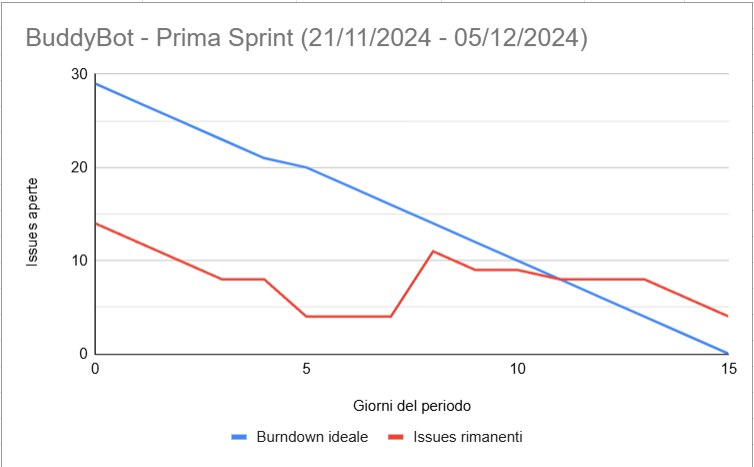
\includegraphics[width=\textwidth]{Burndown ideale - primoperiodo.jpg}
    \caption{Diagramma di Burndown del primo periodo} 
    \label{fig: Diagramma di Burndown del primo periodo}
\end{figure}
\newpage
\begin{figure}[h] 
    \centering
    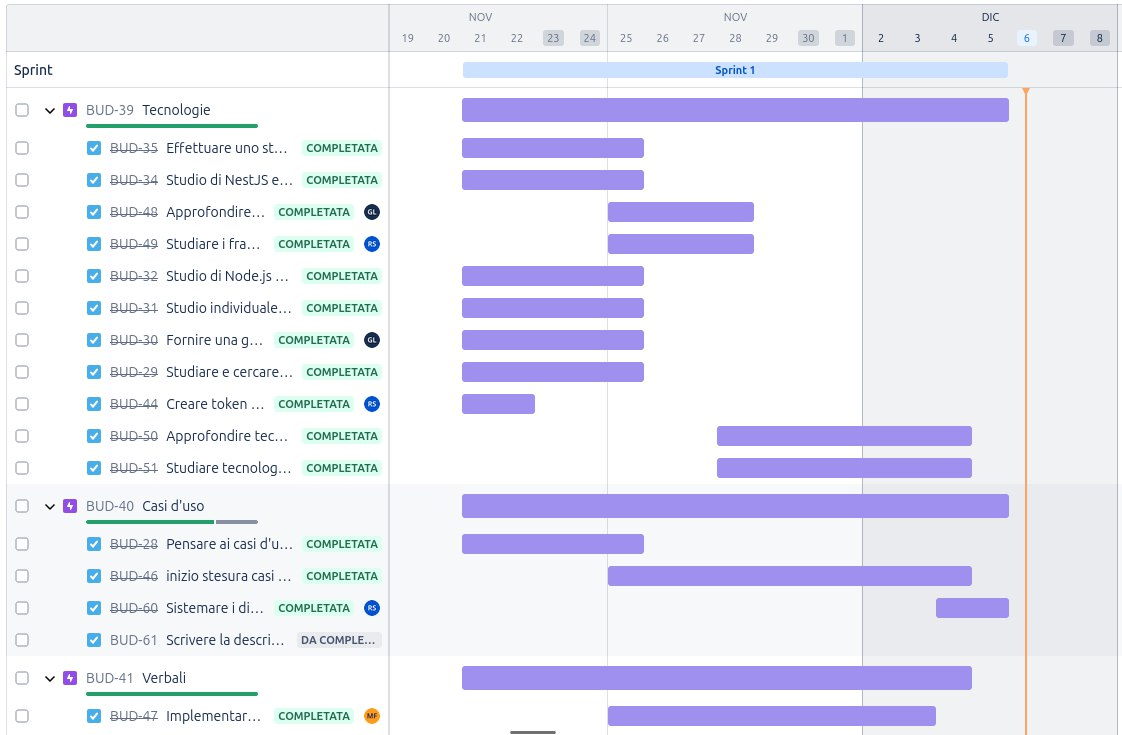
\includegraphics[width=\textwidth]{Diagramma di Gannt(prima parte)primoperiodo.jpg}
    \caption{Diagramma di Gantt primo periodo dal 12/11/204 al 5/12/2024: prima parte} 
    \label{fig: Diagramma di Gantt primo periodo dal 12/11/204 al 5/12/2024: prima parte}
\end{figure}
\newpage


\begin{figure}[h] 
    \centering
    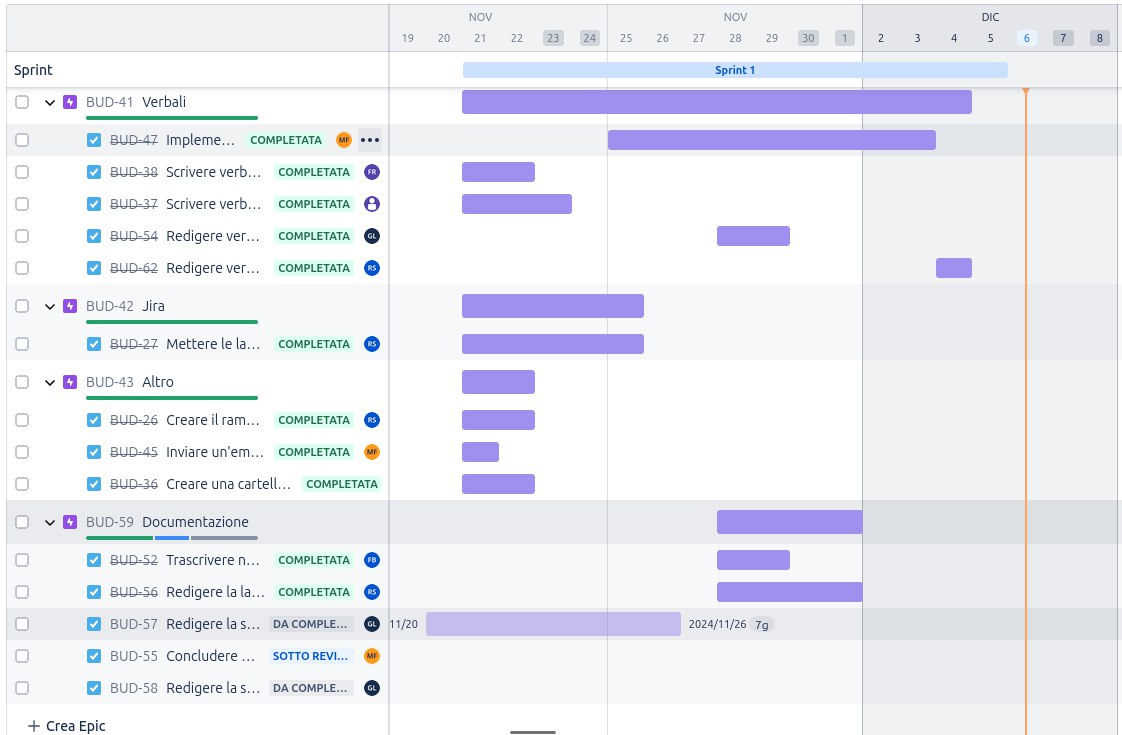
\includegraphics[width=\textwidth]{Diagramma di Gannt(seconda parte)primoperiodo.jpg}
    \caption{Diagramma di Gantt primo periodo dal 12/11/204 al 5/12/2024: seconda parte} 
    \label{fig: Diagramma di Gantt primo periodo dal 12/11/204 al 5/12/2024: seconda parte}
\end{figure}

\newpage
\subsubsubsection{Secondo periodo}
\begin{table}[h!]
    \centering
    \renewcommand{\arraystretch}{1.5} % Aumenta l'altezza delle righe
    \begin{tabularx}{\textwidth}{|X|X|}\hline
    \rowcolor[HTML]{FFD700} 
    \textbf{Data di inizio} & \textbf{Data di fine} \\ \hline
    06/12/2024 & 19/12/2024 \\ \hline
    \end{tabularx}
    \caption{Secondo periodo dedicato alla RTB}
\end{table}
Nel secondo periodo di lavoro, che va dal 6 dicembre al 19 dicembre 2024 e coincide con la seconda \textit{sprint}, abbiamo continuato a lavorare sull’\emph{Analisi dei casi d’uso}, identificando e documentando i punti chiave emersi sia nel confronto con il \emph{proponente} sia nel dialogo con il professore Cardin.\\
Abbiamo iniziato la trascrizione dei \emph{requisiti}, trasformando i \emph{casi d’uso} in specifiche tecniche e funzionali.\\
Per quanto riguarda le tecnologie, abbiamo confermato la nostra scelta e le abbiamo validate iniziando ad includerle nel \emph{PoC}, che rappresenta un primo prototipo. Il PoC, avviato durante questo sprint, risponde a domande riguardanti dati presenti su \emph{GitHub}, \emph{Confluence} e \emph{Jira}, presenta una struttura organizzata in classi e modulare, dispone di header che forniscono istruzioni al browser, che saranno incrementati successivamente, e affronta alcune problematiche legate alla ricerca di similarità che saranno risolte con una migliore strutturazione dei dati. \\
Infiine, abbiamo iniziato a compilare una lista di documenti di riferimento chiave e li abbiamo organizzati in \emph{Confluence}, \emph{Jira} e \emph{GitHub}, con l’obiettivo di garantire un contesto chiaro e accessibile per il team.

\newpage

\begin{figure}[h] 
    \centering
    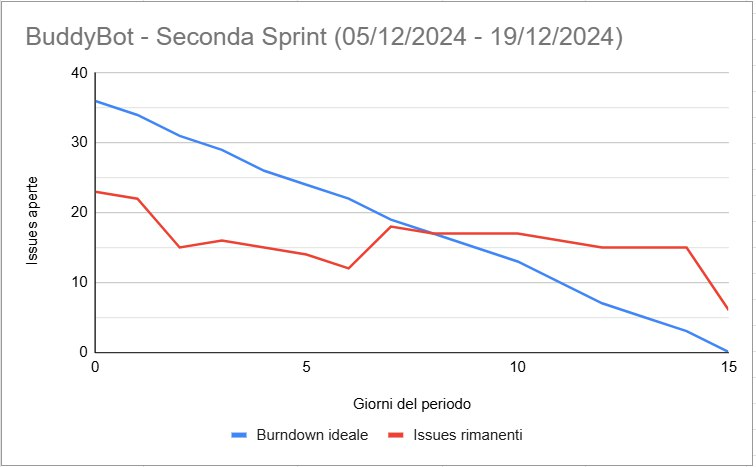
\includegraphics[width=\textwidth]{Burndown ideale - secondoperiodo.jpg}
    \caption{Diagramma di Burndown del secondo periodo} 
    \label{fig: Diagramma di Burndown del secondo periodo}
\end{figure}

\newpage

\begin{figure}[h] 
    \centering
    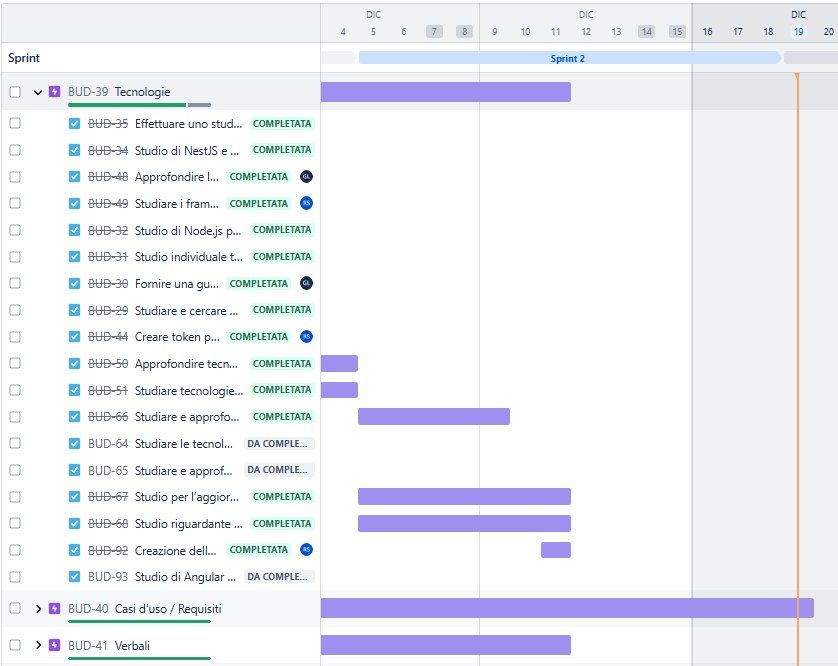
\includegraphics[width=\textwidth]{Diagramma di Gannt(prima parte)secondoperiodo.jpg}
    \caption{Diagramma di Gantt secondo periodo dal 06/12/2024 - 19/12/2024: prima parte} 
    \label{fig: Diagramma di Gantt primo periodo dal 06/12/2024 - 19/12/2024: prima parte}
\end{figure}

\newpage

\begin{figure}[h] 
    \centering
    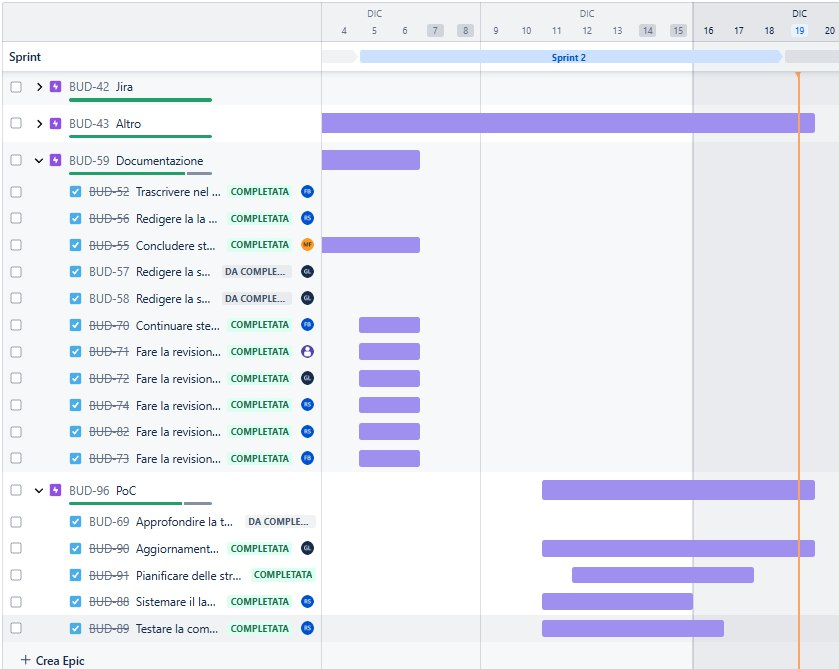
\includegraphics[width=\textwidth]{Diagramma di Gannt(seconda parte)secondoperiodo.jpg}
    \caption{Diagramma di Gantt secondo periodo dal 06/12/2024 - 19/12/2024: seconda parte} 
    \label{fig: Diagramma di Gantt primo periodo dal 06/12/2024 - 19/12/2024: seconda parte}
\end{figure}

\newpage